\documentclass[a4paper,11pt]{article}
\usepackage[utf8]{inputenc}
\usepackage[T1]{fontenc}
\usepackage[french]{babel}
\usepackage{graphicx}
\usepackage{lipsum}
\usepackage[a4paper]{geometry}
\usepackage{wallpaper}
\usepackage{libertine}
\usepackage{csquotes}
\usepackage{fancyhdr}
\usepackage{vmargin}
\usepackage{hyperref}
\usepackage[colorinlistoftodos]{todonotes}
\usepackage{titlesec}
\usepackage{array}



\makeatletter
\def\clap#1{\hbox to 0pt{\hss #1\hss}}%
\def\ligne#1{%
\hbox to \hsize{%
\vbox{\centering #1}}}%
\def\haut#1#2#3{%
\hbox to \hsize{%
\rlap{\vtop{\raggedright #1}}%
\hss
\clap{\vtop{\centering #2}}%
\hss
\llap{\vtop{\raggedleft #3}}}}%
\def\bas#1#2#3{%
\hbox to \hsize{%
\rlap{\vbox{\raggedright #1}}%
\hss
\clap{\vbox{\centering #2}}%
\hss
\llap{\vbox{\raggedleft #3}}}}%
\def\maketitle{%
\thispagestyle{empty}\vbox to \vsize{%
\haut{}{\@blurb}{}
\vfill
\vspace{1cm}
\begin{flushleft}
\usefont{OT1}{ptm}{m}{n}
\huge \@title
\end{flushleft}
\par
\hrule height 4pt
\par
\begin{flushright}
\usefont{OT1}{phv}{m}{n}
\Large \@author
\par
\end{flushright}
\vspace{1cm}
\vfill
\vfill
\bas{}{\@location, le \@date}{}
}%
\cleardoublepage
}
\def\date#1{\def\@date{#1}}
\def\author#1{\def\@author{#1}}
\def\title#1{\def\@title{#1}}
\def\location#1{\def\@location{#1}}
\def\blurb#1{\def\@blurb{#1}}
\Large{\date{\today}}
\author{}
\title{}
\location{Rennes}\blurb{}
\makeatother
\title{\LARGE{Projet Modélisation et Programmation Orientée Objet}}
\author{Frank \textsc{Chassing} et Amandine \textsc{Fouillet}}
\location{Rennes}
\blurb{%
\large{INSA de Rennes\\
\textbf{Rapport de conception}}
}%


\begin{document}
\maketitle
\tableofcontents
\newpage
\section*{Introduction}
\addcontentsline{toc}{section}{Introduction}
Dans le cadre des cours de Programmation Orientée Objet et de Modélisation et Conception de Logiciels, nous sommes amenés à réaliser un jeu pour ordinateur semblable au jeu Small World. Dans la première partie de ce projet, nous avons réalisé la modélisation du problème grâce à divers diagrammes UML pour, dans un second temps, réaliser l'implémentation du jeu. \\

Le jeu à réaliser est un jeu tour-a-tour dans lequel chaque joueur dirige un peuple qui contient plusieurs unités. Le but du jeu est de gérer les unités sur une carte du monde pour obtenir le plus de points possible à la fin d'un certain nombre de tours. Pour gagner il faut contrôler le plus de cases possibles en attaquant les unités adverses, en défendant son territoire et en se déplaçant sur les cases vides. Dans notre implémentation du jeu, deux joueurs s'opposerons, ils pourront choisir trois peuples différents : les elfs, les orcs et les nains et se déplacer sur trois types de cases différents : la forêt, le désert, la montagne et la plaine.\\

Ce rapport présente le travail réalisé lors de la phase de modélisation au cours de laquelle plusieurs diagrammes ont été réalisés afin de décrire les différents aspects du jeu. Ce rapport est découpé dans l'optique de découvrir toutes les phases du jeu. Ainsi, dans un premier temps nous étudierons la phase de création d'une partie grâce aux diagrammes de cas d'utilisation, d'activité et de séquence. Puis nous étudierons le déroulement d'une partie, d'un tour de jeu et d'un combat la encore avec des diagrammes d'interaction, d'activité et de cas d'utilisation. Pour résumer et conclure sur la modélisation du jeu, nous finirons par détailler le diagramme de classe réalisé ainsi que les différents patrons de conception utilisés.
\newpage
\section{Création de la partie}
\lipsum[1]
\subsection{Diagramme de cas d'utilisation}
\begin{figure}[h!]
\fbox{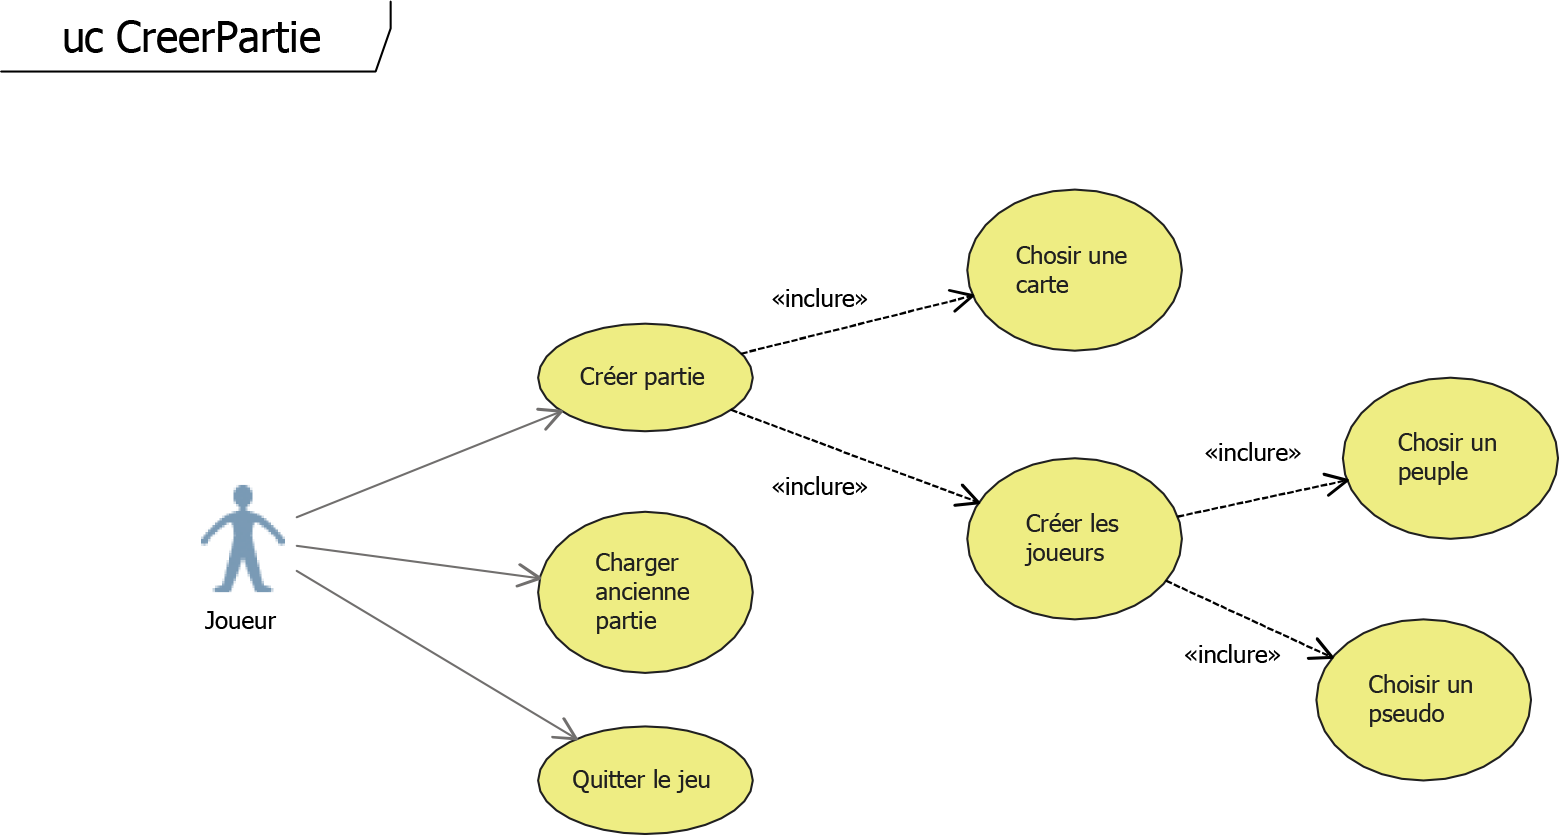
\includegraphics{ucCreerPartie.png}}
\caption{Cas d'utilisation - Créer une Partie}
\end{figure}
\newpage
\subsection{Diagramme d'activité}
\begin{figure}[ht!]
\fbox{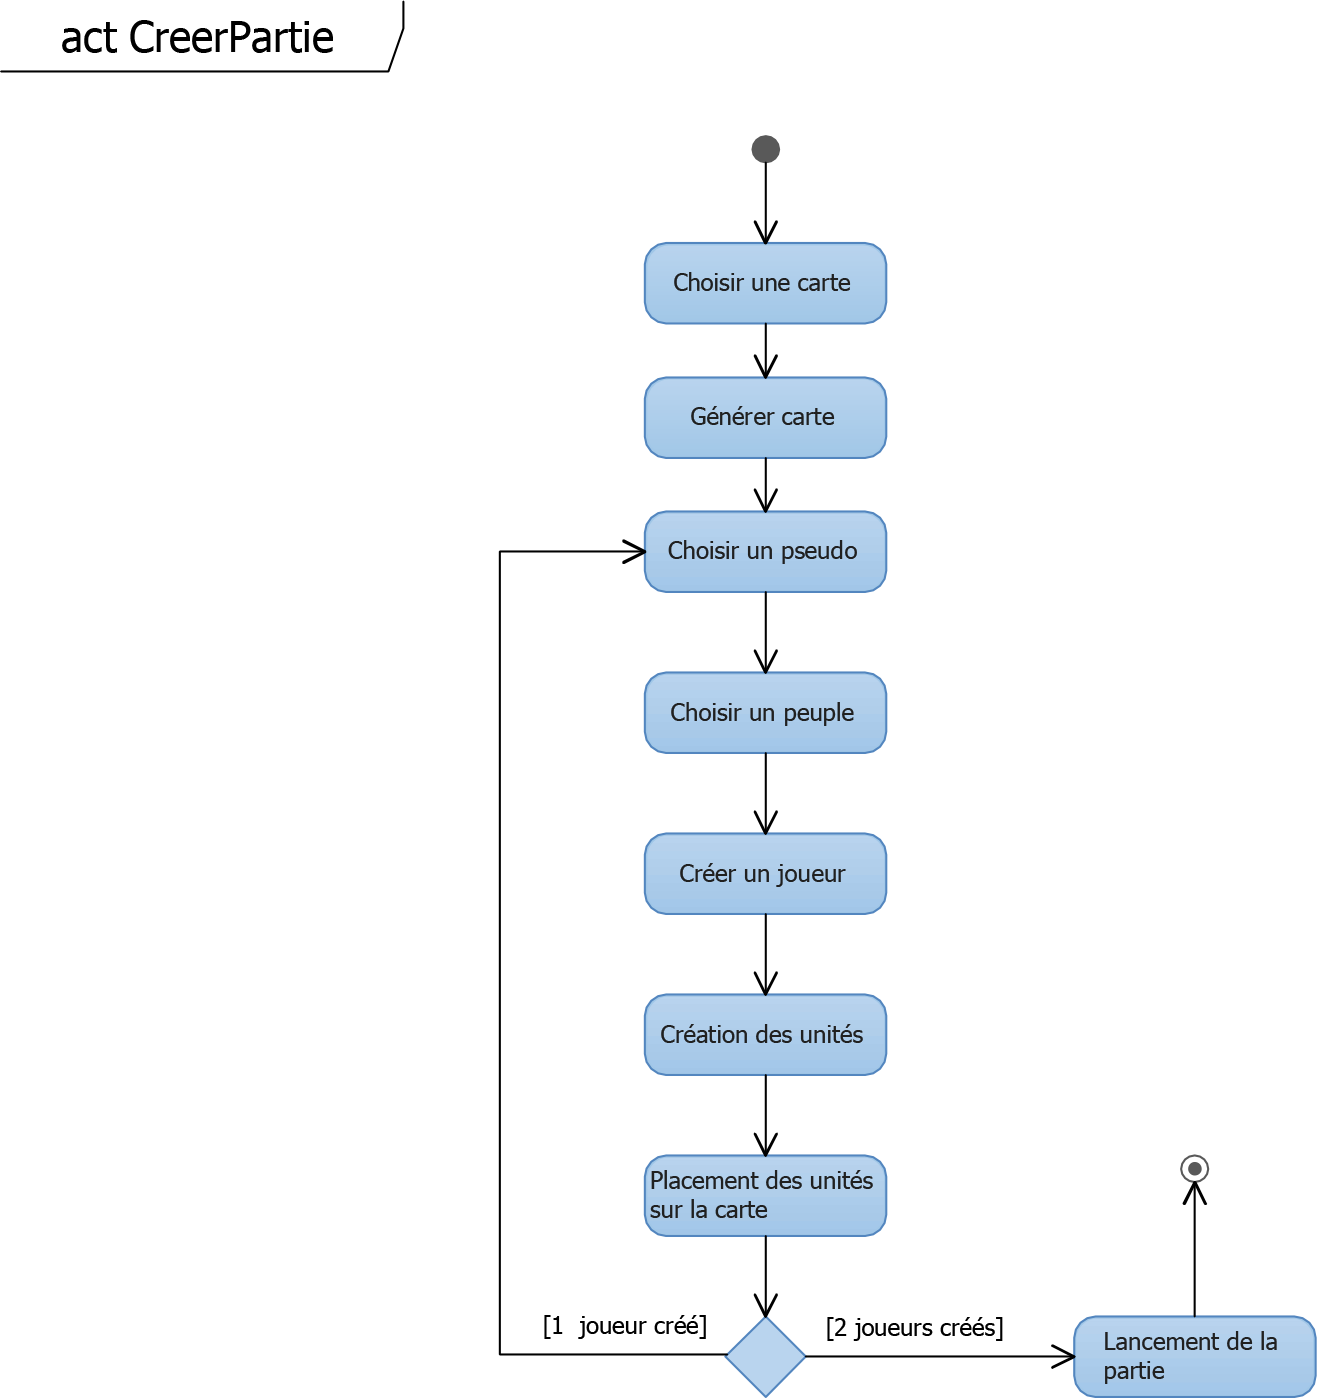
\includegraphics{actCreerPartie.png}}
\caption{Cas d'utilisation - Créer une Partie}
\end{figure}
\newpage
\subsection{Diagramme de séquence}
\begin{figure}[ht!]
\fbox{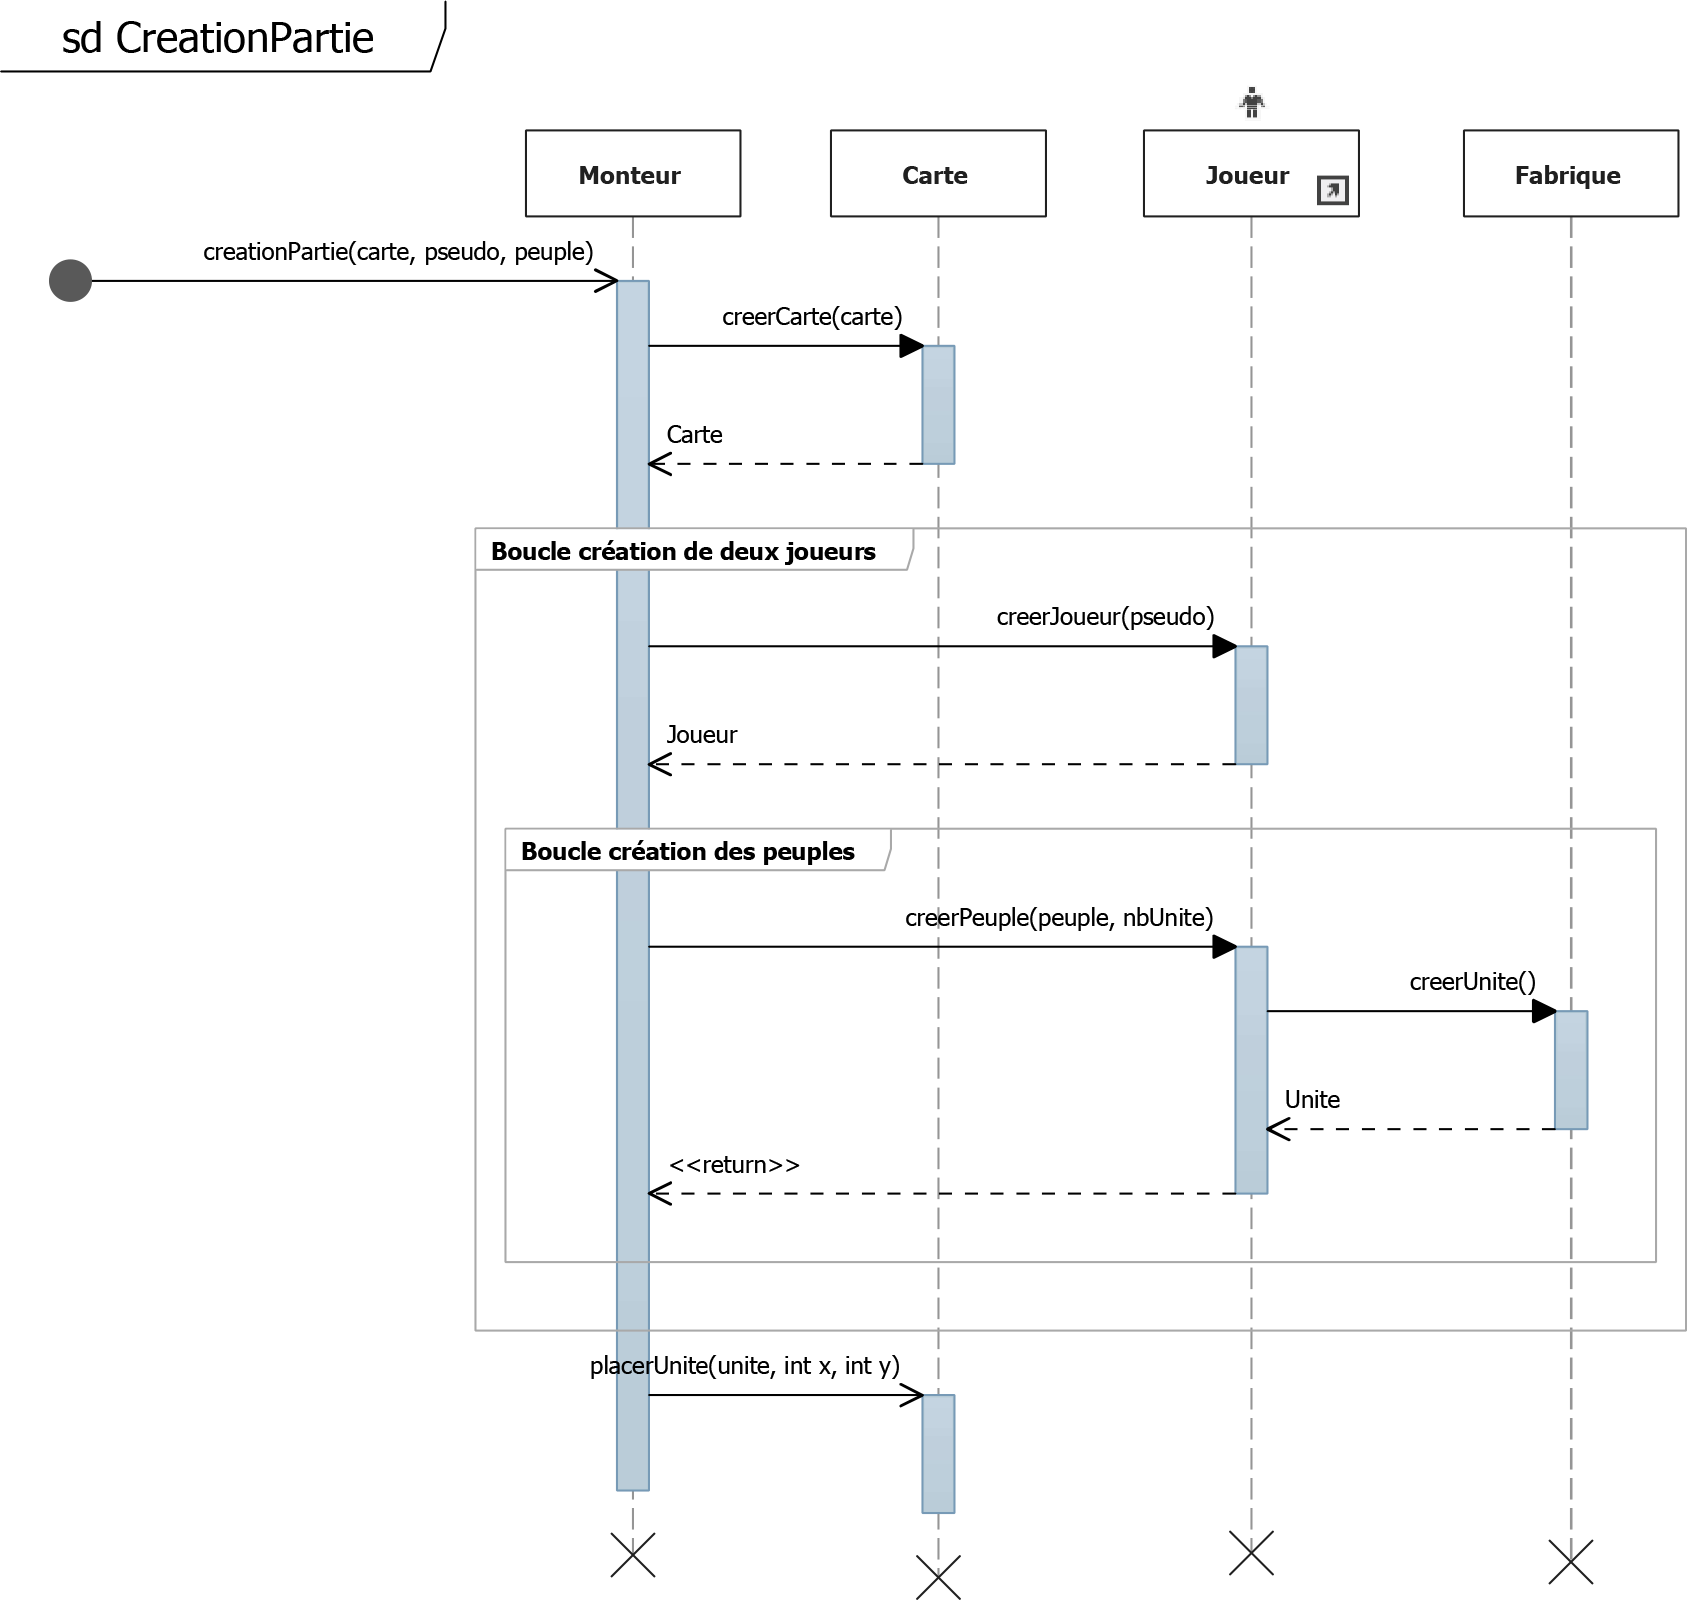
\includegraphics{sqCreerPartie.png}}
\caption{Cas d'utilisation - Créer une Partie}
\end{figure}

\newpage
\section{Déroulement d'une partie}
\lipsum[1]
\begin{figure}[ht!]
\fbox{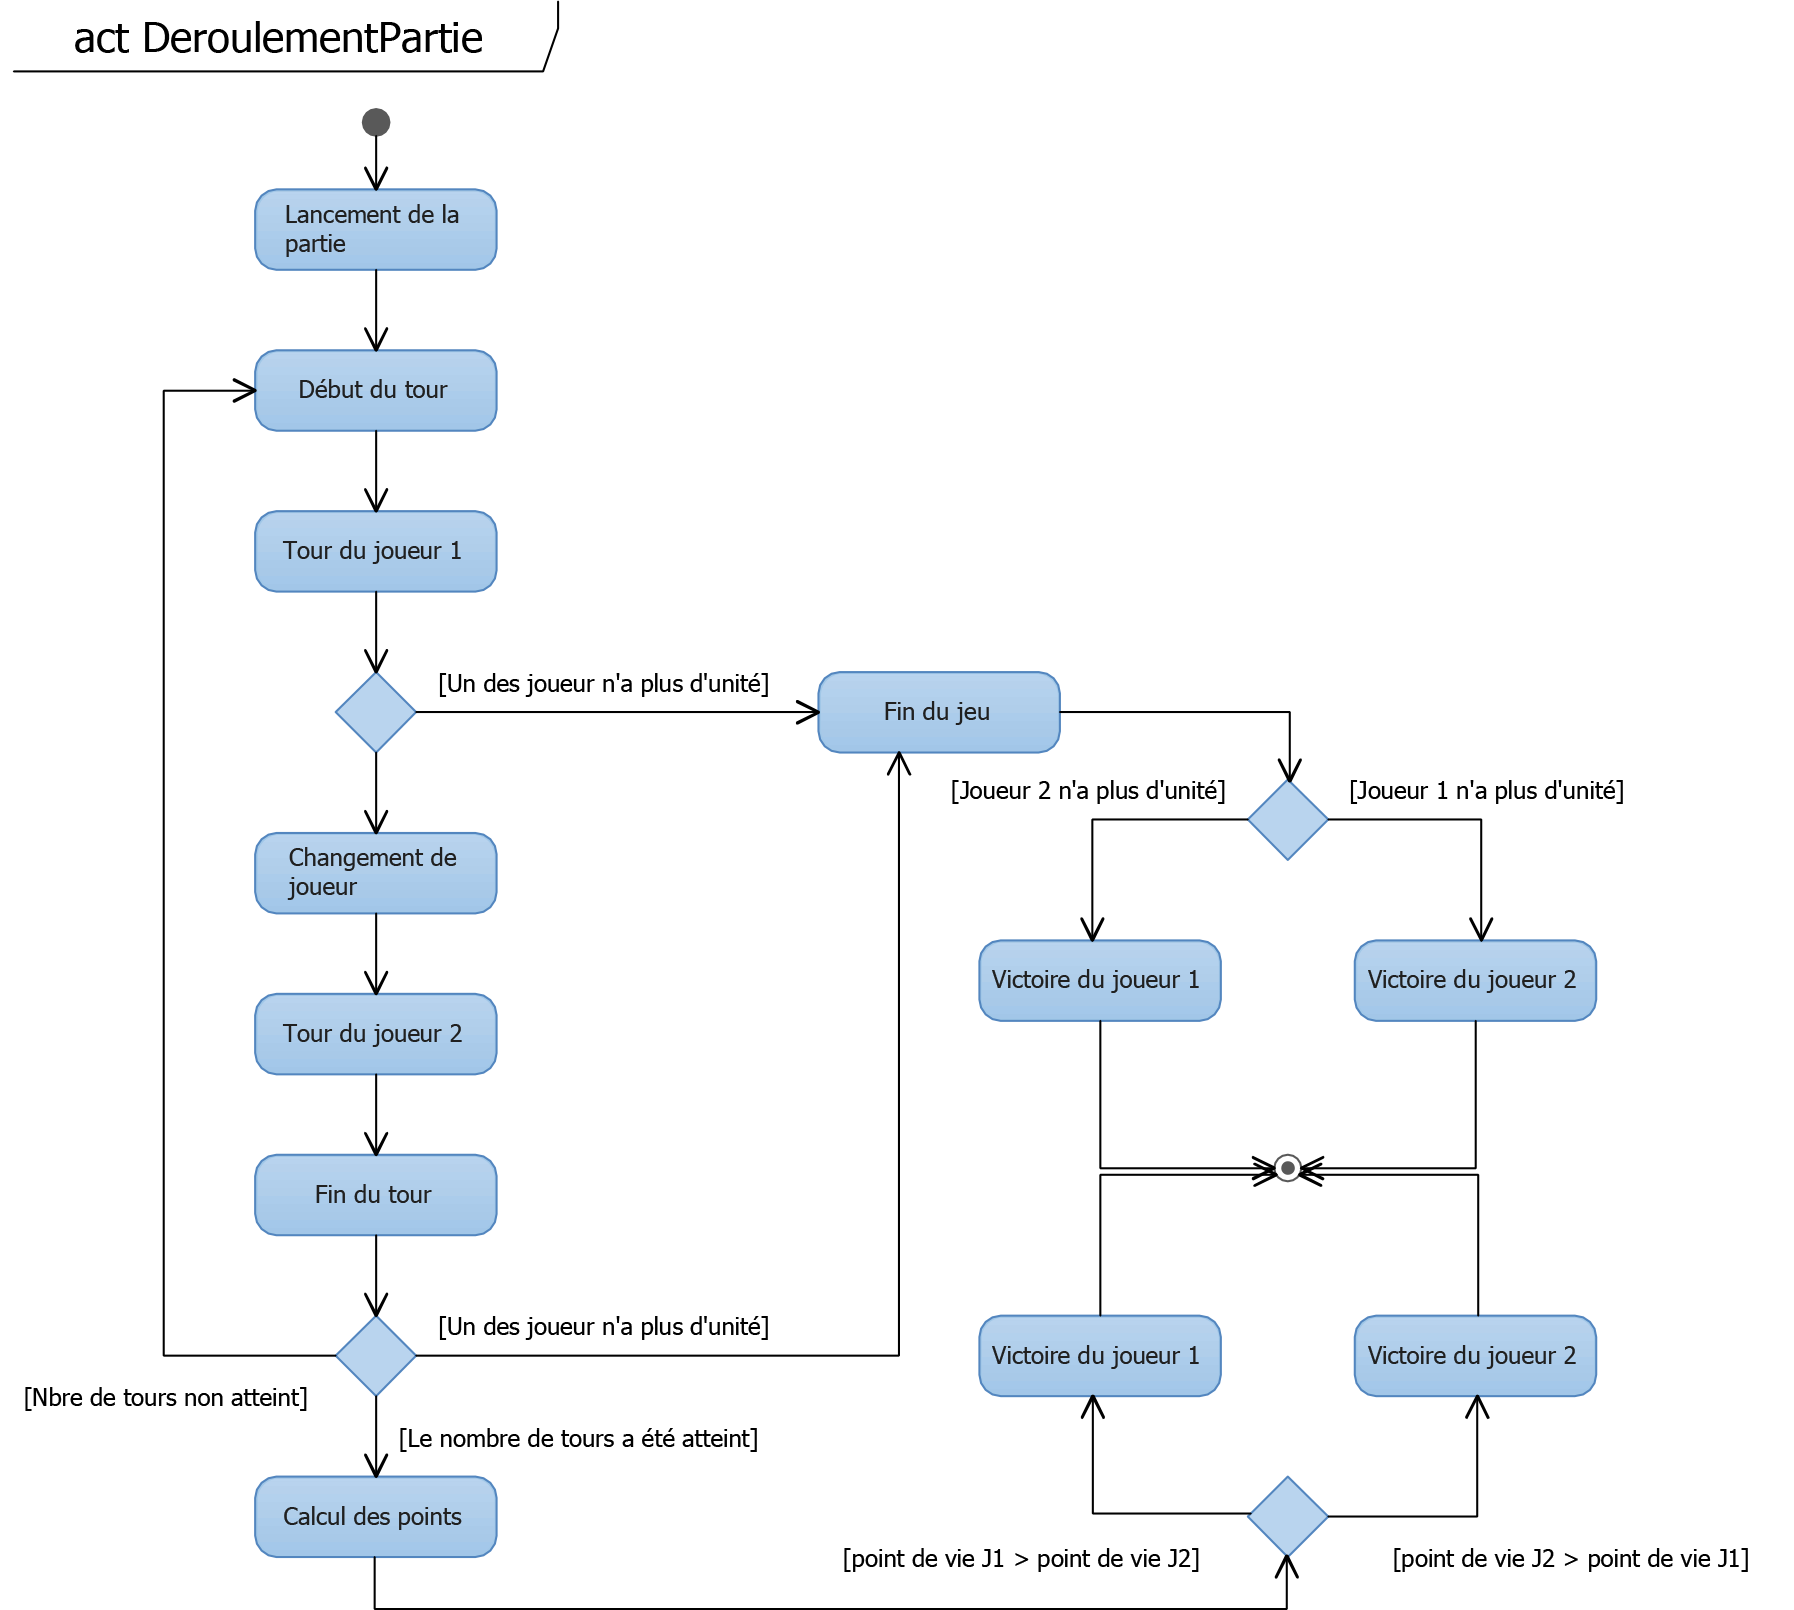
\includegraphics{actDeroulementPartie.png}}
\caption{Cas d'utilisation - Créer une Partie}
\end{figure}
\newpage
\subsection{Déroulement d'un tour de jeu}
\lipsum[1]
\subsubsection{Diagramme de cas d'utilisation}
\begin{figure}[ht!]
\fbox{\includegraphics{ucTourDeJeu.png}}
\caption{Cas d'utilisation - Créer une Partie}
\end{figure}
\newpage
\subsubsection{Diagrammes d'activités}
\begin{figure}[ht!]
\fbox{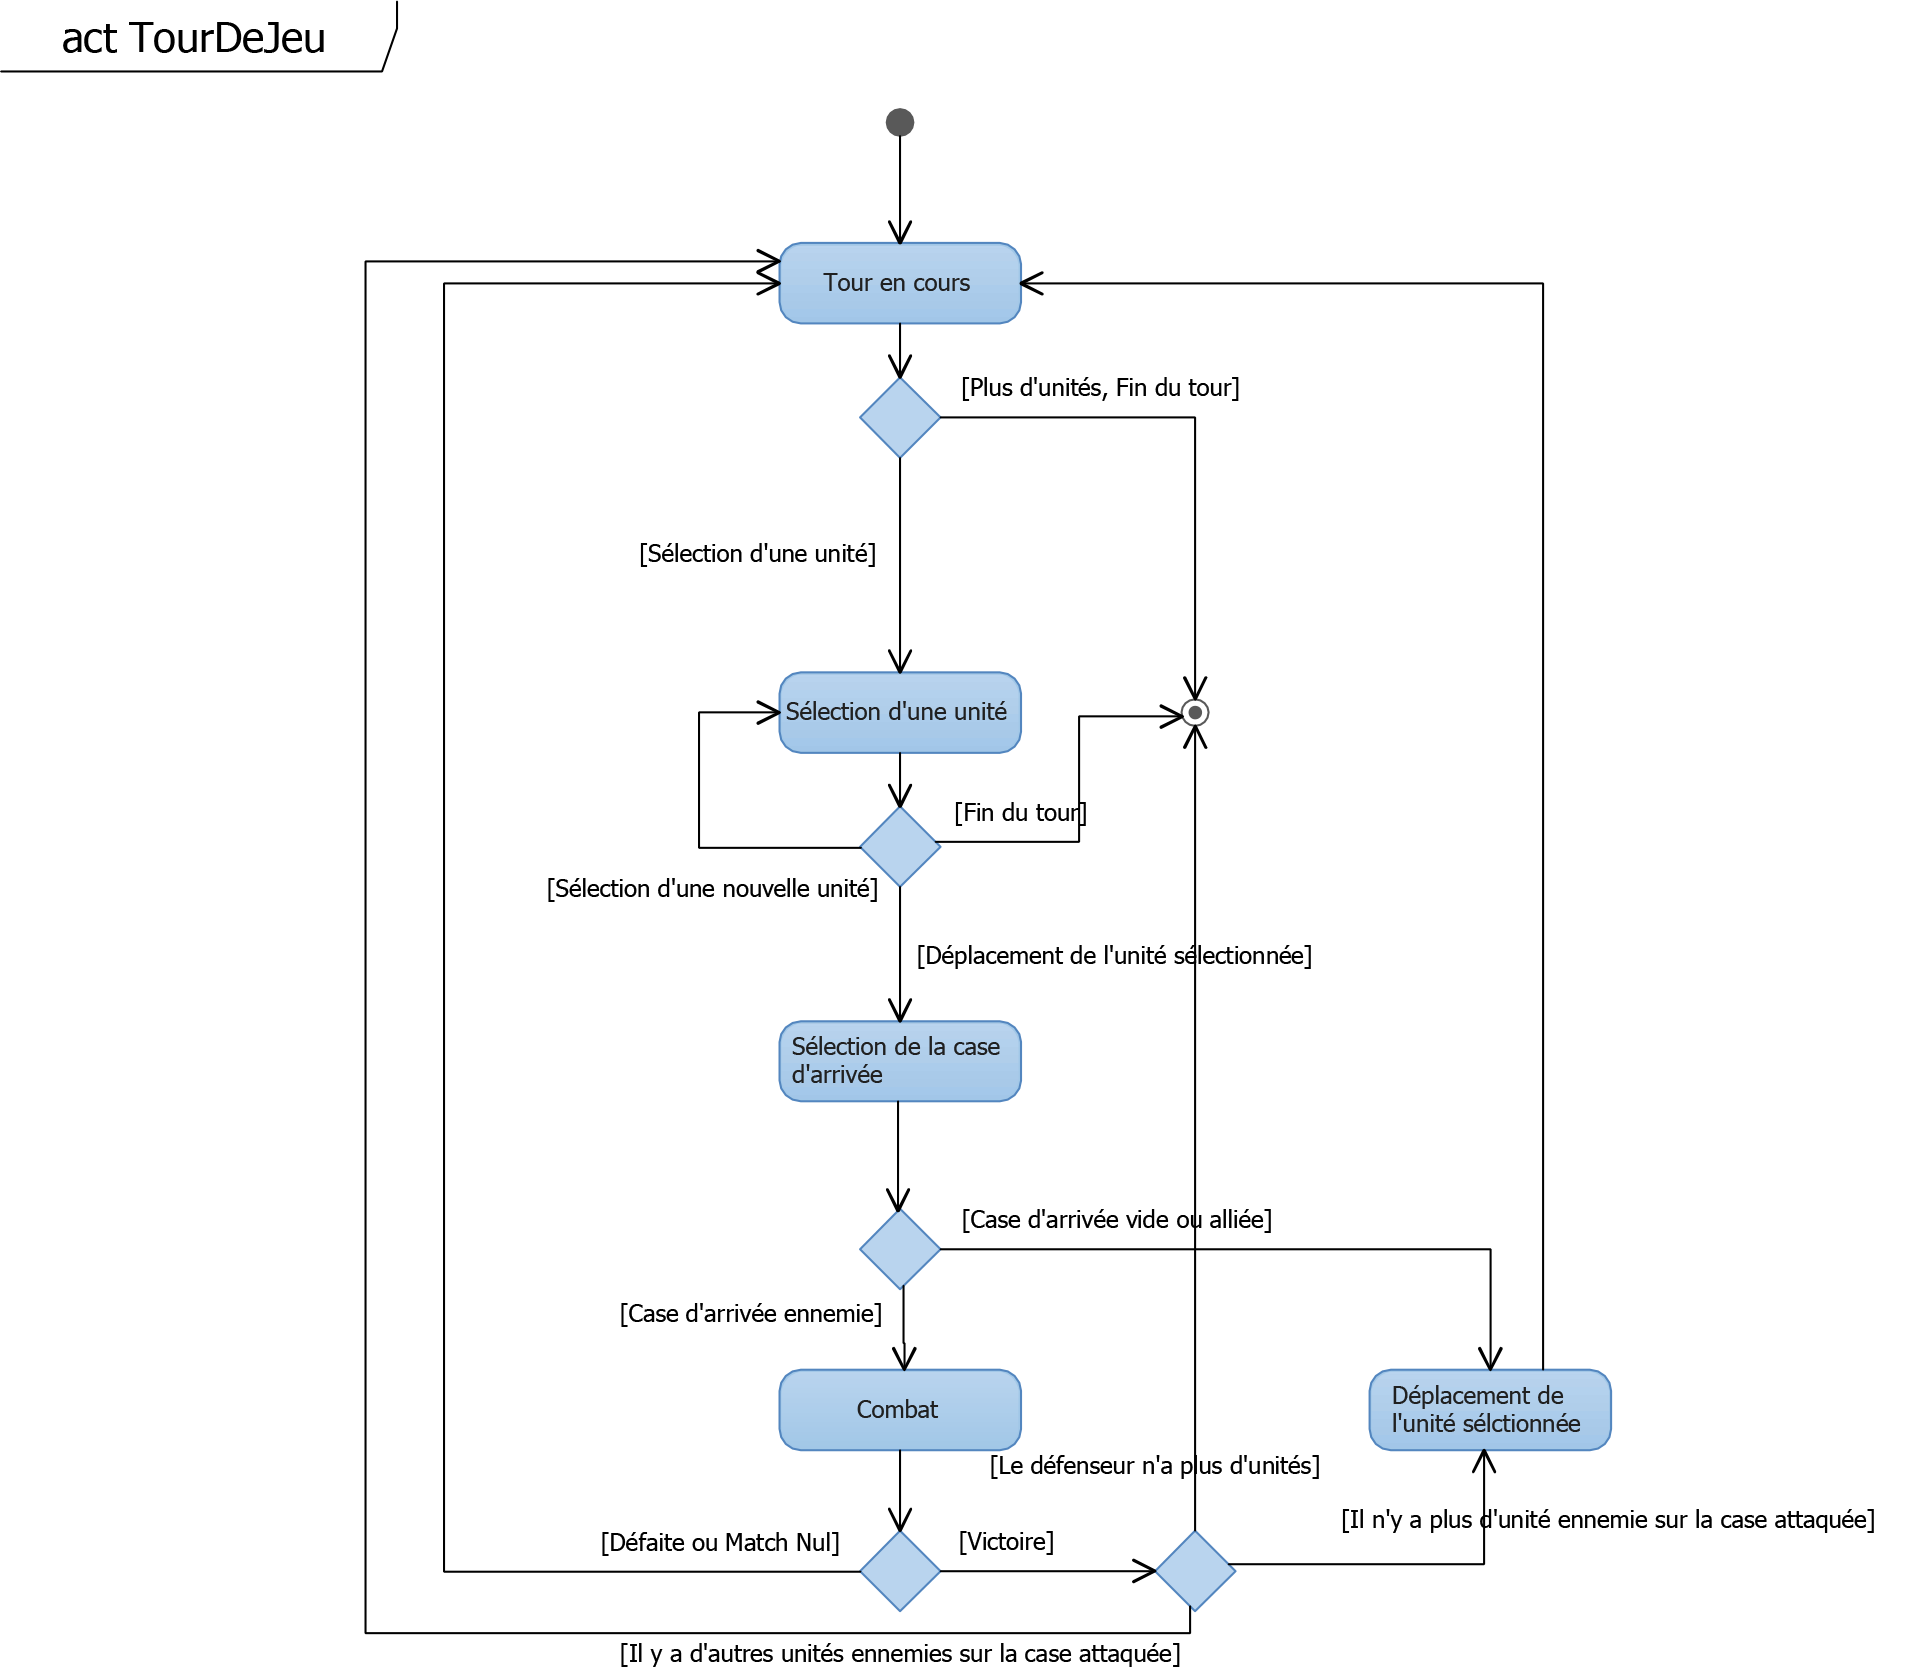
\includegraphics{actTourDeJeu.png}}
\caption{Cas d'utilisation - Créer une Partie}
\end{figure}
\newpage
\subsection{Déroulement d'un combat}
\begin{figure}[ht!]
\fbox{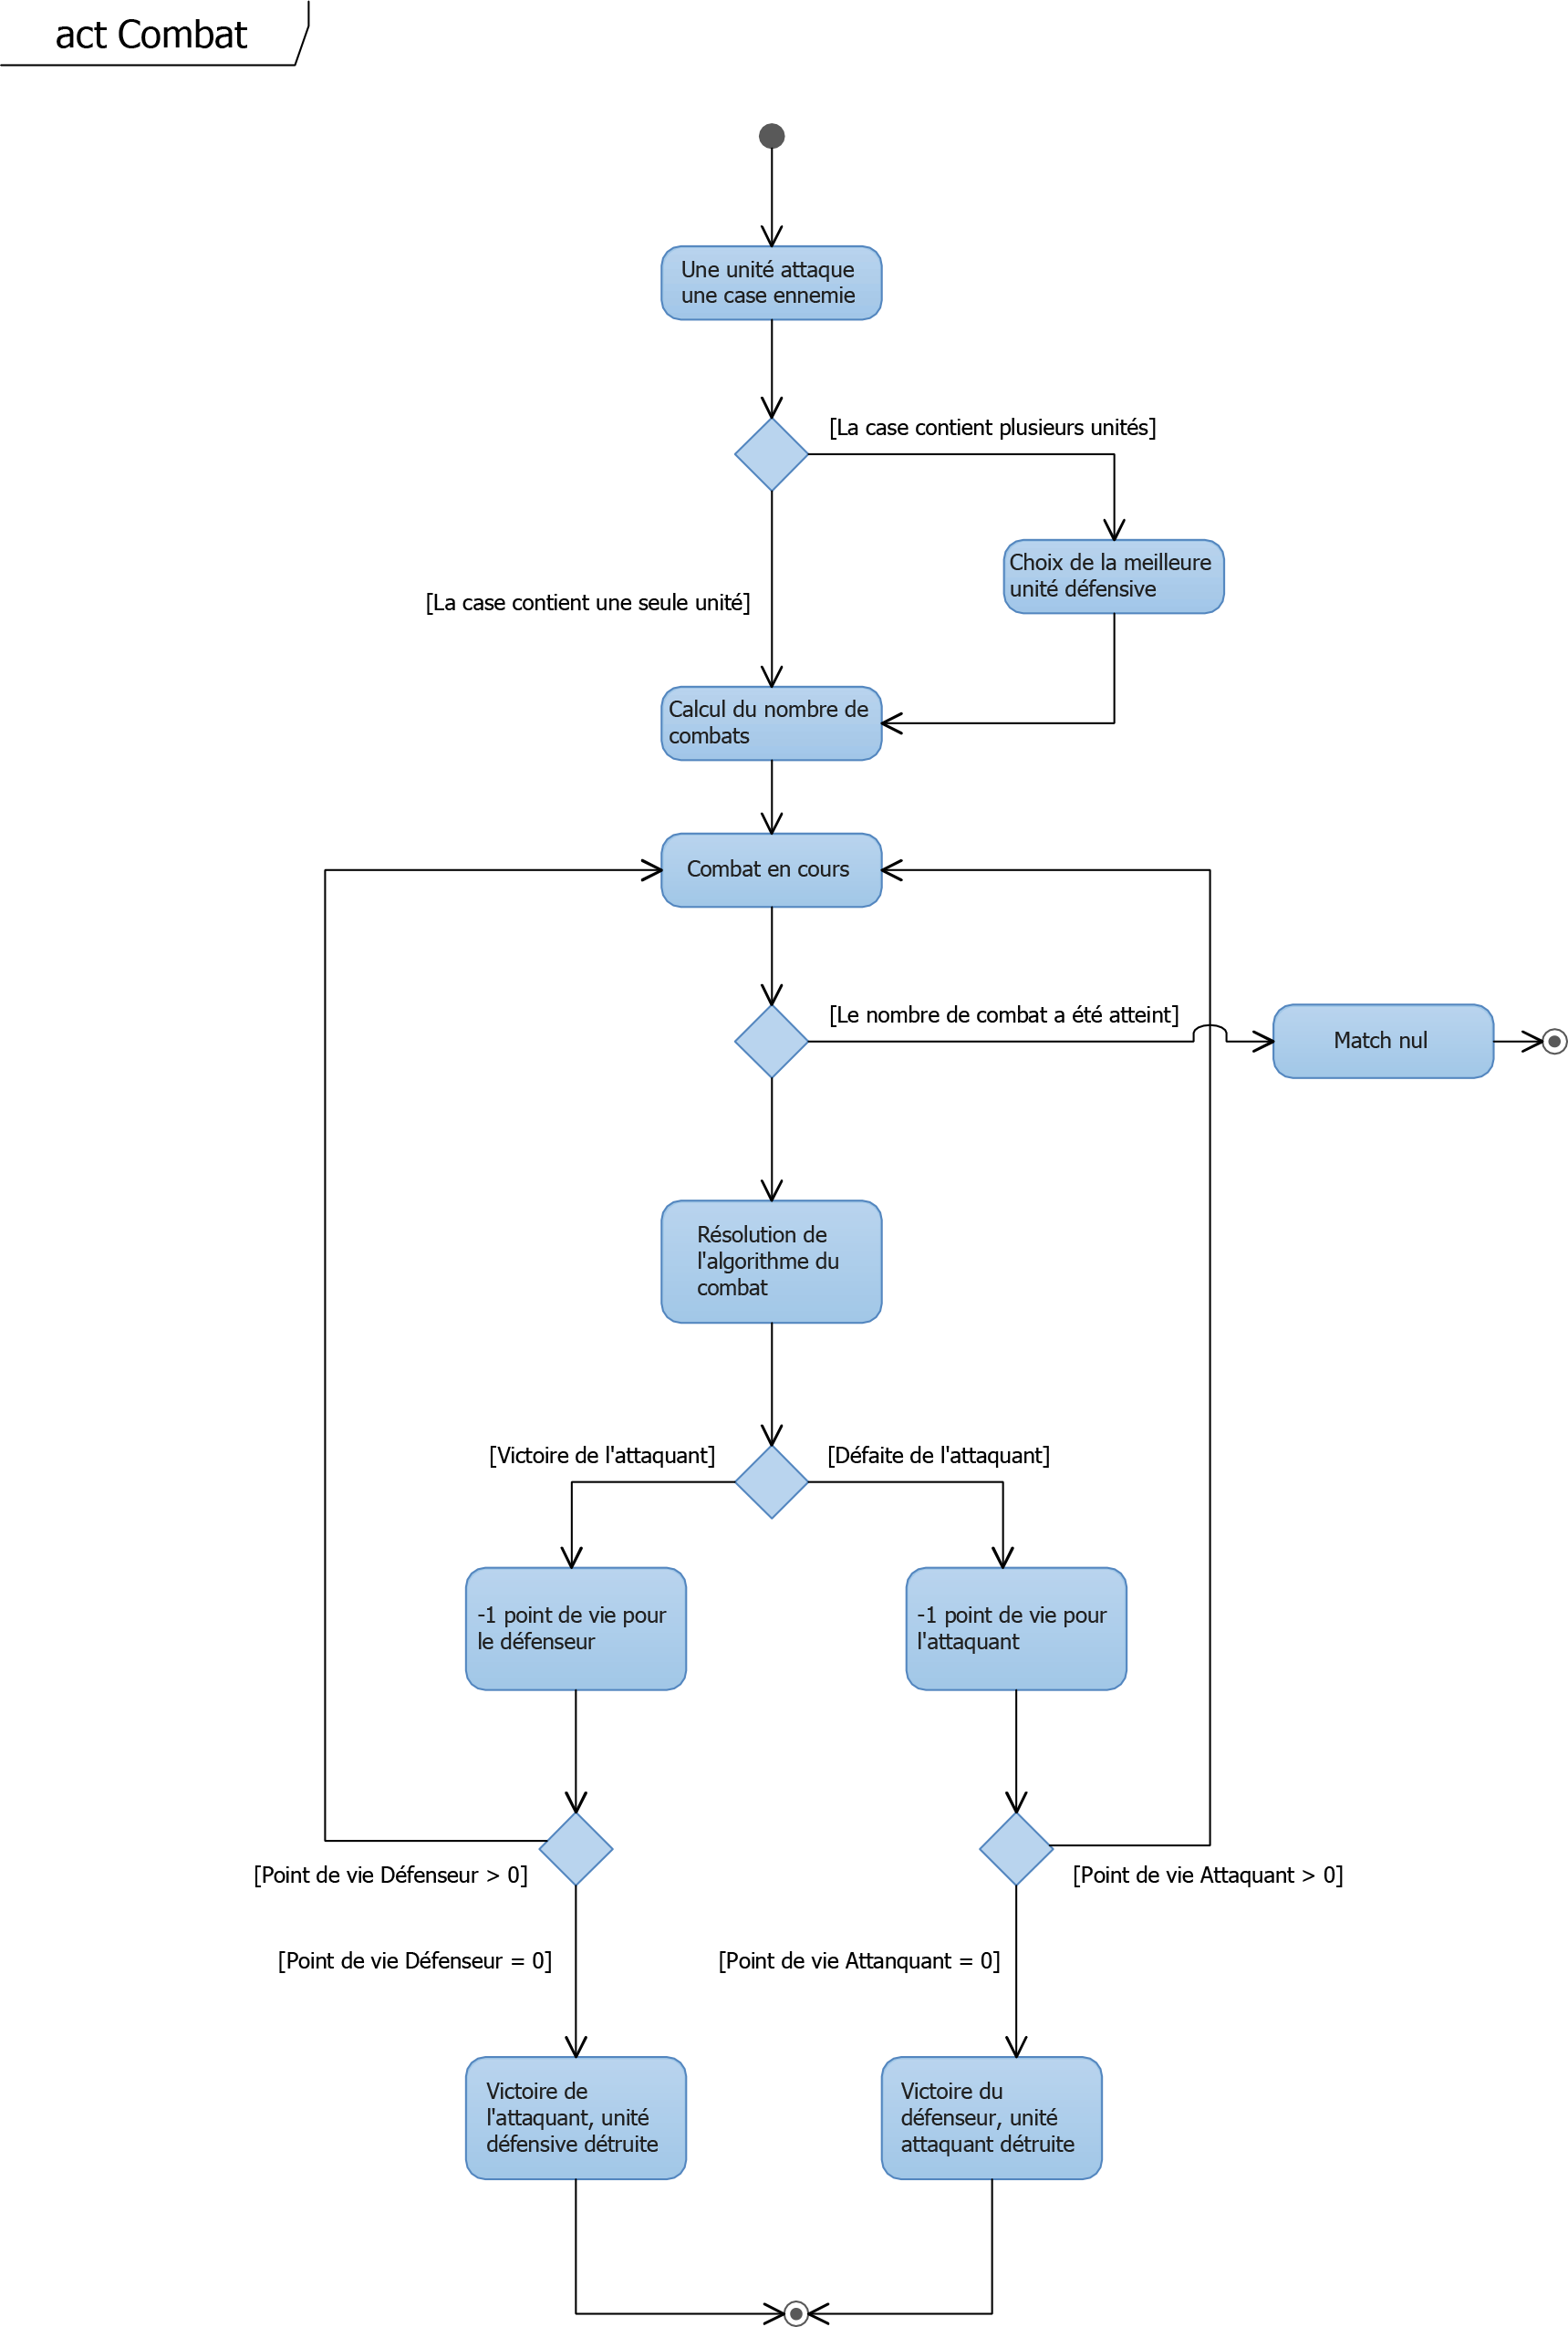
\includegraphics[height=18cm]{actCombat.png}}
\caption{Cas d'utilisation - Créer une Partie}
\end{figure}

\newpage
\section{Diagramme de classe}
\lipsum[1]
\subsection{Modélisation globale}
\subsection{Patrons de conception}
\subsubsection{Fabrique}
\subsubsection{Monteur}
\subsubsection{Poids-mouche}
\subsubsection{Stratégie}


\newpage
\section*{Conclusion}
\addcontentsline{toc}{section}{Conclusion}
\lipsum[1-2]
\end{document}